\section{ETL}\label{sec:ETL}
The data foundation for this project relies on two sources, refer section \ref{sec:datafound}. Extract-Transform-Load(ETL) is an important phase for integrating these two sources of information into the data warehouse while ensuring a uniform data-representation. A preprocessing procedure fills static support-tables and dimensions with data. The data foundation contains data for car information and part of GPS Fact. After the preliminary data is loaded, a number of post-processing procedures fills the remaining tables in the data warehouse with data.

\begin{figure}[tb]
\centering
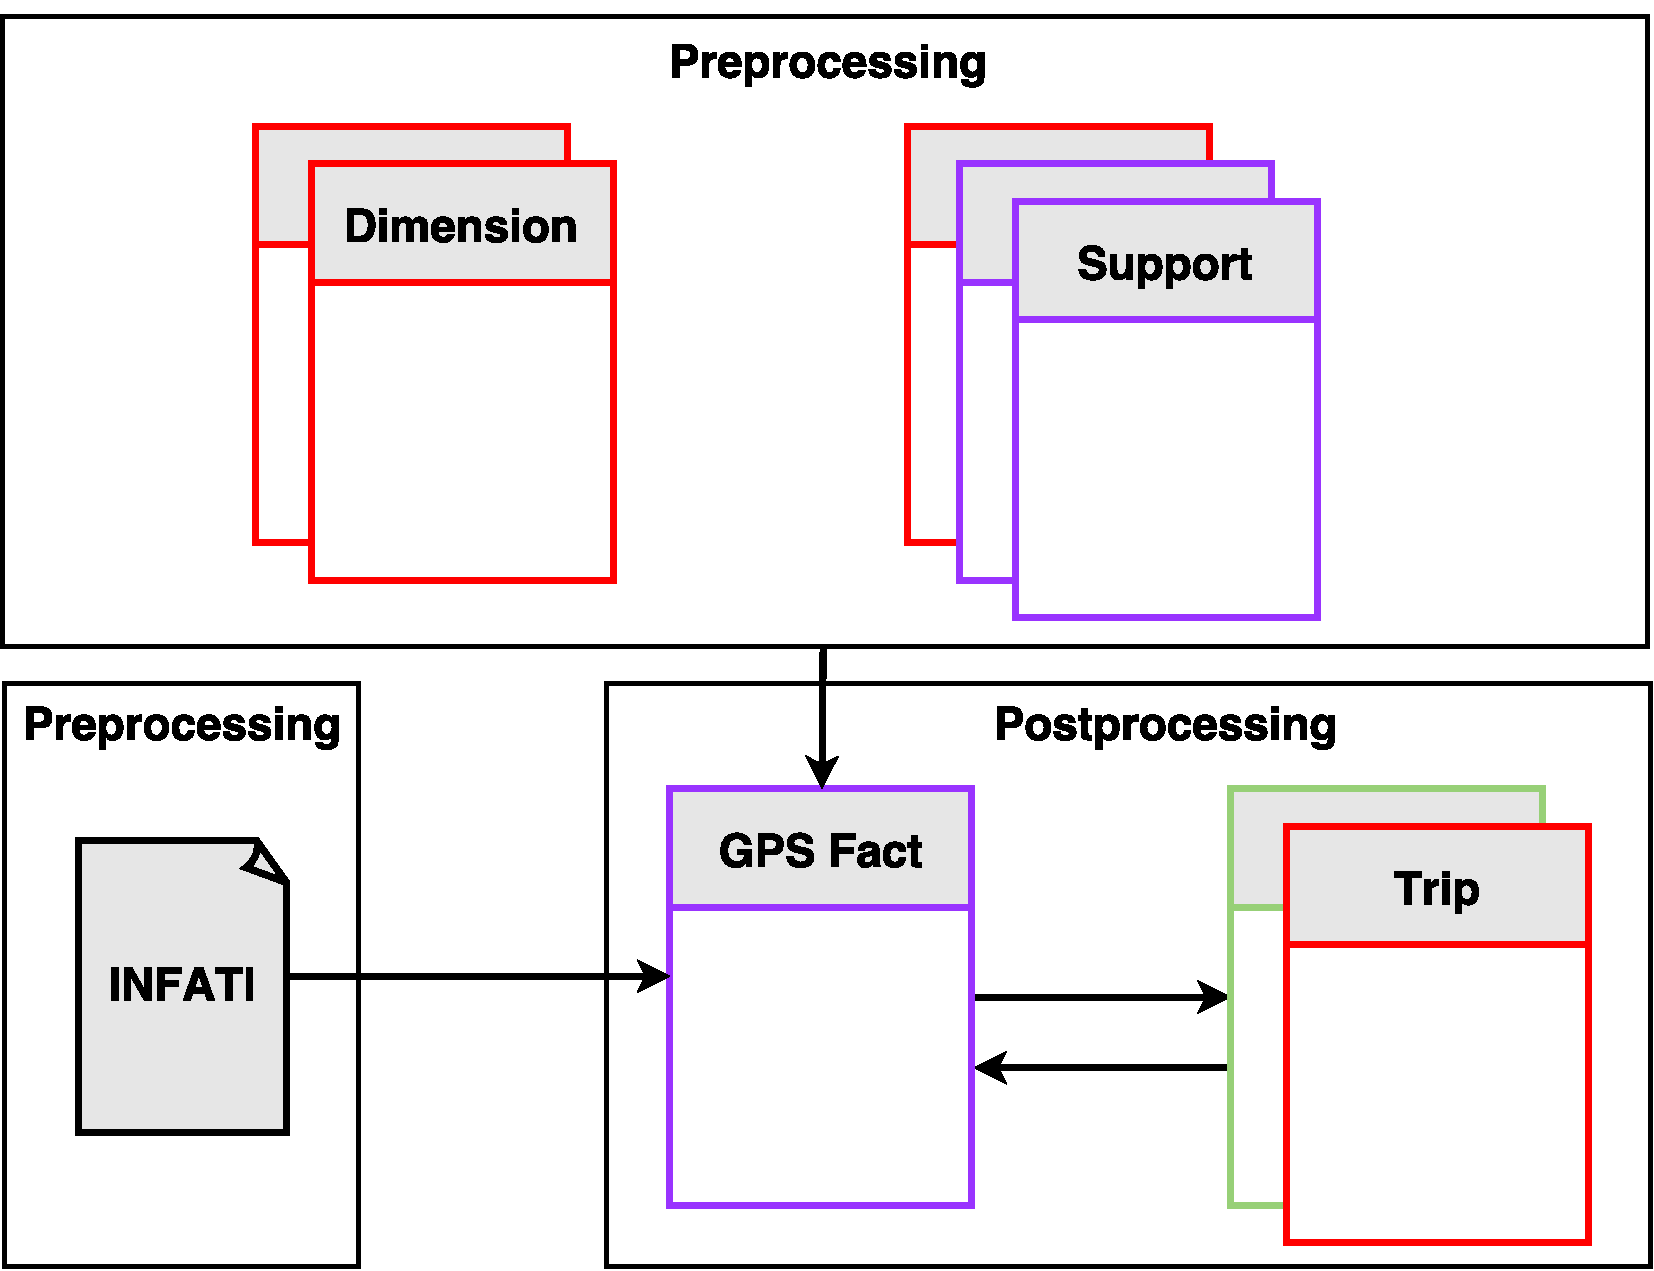
\includegraphics[width=0.465\textwidth]{Pictures/ETL}
\caption{Dataflow throughout the ETL process}
\label{fig:etl}
\end{figure}

The INFATI project\cite{art:INFATI} uses a digital roadmap from OpenStreetMap\cite{osm}. The same digital roadmap is used for this project. A few modifications is introduced, like storing the column \textit{direction} as a smallint instead of a textual representation. 

The INFATI dataset\cite{art:INFATI} contains 17 columns of data, separated by a varying number of spaces. Due to the natural challenges of map-matching, some entries contain only 14 columns of data. This causes the dataset to have problems with trailing zeros when loading with a space-separator. To ease the ETL process, a script has to be made for altering the separator. In this example \# is used, and whenever a row was not map-matched, three \#'s are appended to that row.

INFATI coordinate-sets are stored in Universal Transverse Mercator (UTM 32) format. This system is build on GPS, and a transformation from UTM to lattitude and longitude are needed. Coordinate-sets are stored as points, lines or polygons and stored in the data warehouse as PostGIS\cite{postgis} geometries. These geometries has to be assigned the correct spatial reference system identifier(SRID), otherwise they will refer to an incorrect positions. INFATI is logged in UTM32 North format, which has SRID 23032\cite{UTM32N}. Latitude and Longitude format is part of World Geodetic System(WGS), latest edition is WGS84 and has SRID 4326\cite{WGS84}. To transform the format: the geometry is created, assigned the UTM SRID, and transformed into WGS84 latitude longitude format using WGS84 SRID. 

Appropriate data for the support-table \textit{Quality Information} and the dimensions \textit{Date} and \textit{Time} are computed and stored. For \textit{Quality Information} this means storing each combination of HDOP and satellites.

The preprocessing is now complete, and the INFATI data can be loaded into the data warehouse. A car must be created and stored in \textit{Car Information}-table, hereafter the corresponding INFATI-data is loaded into the \textit{GPS Fact}-table. 

Three postprocessing-steps will now fill in measures that will make it possible to determine the cost of a trip. 

The first step is dividing the batch of gpsfacts into trips for each car. Each found trip will be stored in an empty Trip Fact. That TripId will then be assigned the appropriate CarId and an auto-incremented TripId, and the gpsfacts belonging to that calculated trip will be updated with the assigned TripId. This is done by fetching the gpsfact from the data warehouse, and sort them based on their timestamp. A new instance of a trip-class is created, and gpsfacts are continuously stored into this trip-class. When a timestamp is encountered, that is more than three minutes older than the previous, a new trip-class is instantiated. The process then continuous by storing gpsfacts in trip-classes this way, until no more gpsfacts have not been stored in a trip-class. These trip-classes are then used to store tripfacts and update gpsfacts.

The second step is calculating all the measures for all gpsfacts. The process will take one car at a time, fetch all TripIds for that car, go by one trip at a time, fetch the gpsfacts for that trip, calculate the measures for that trip, and update the gpsfacts for that trip with these measures. This is done by fetching all gpsfacts for a certain trip, and sort them based on their timestamp. A loop will then start working from the 2nd entry, and calculate measures based on what happened since the previous entry. It is metrics like acceleration change, and meters driven that will be stored. Once a trip runs out of gpsfacts, these gpsfacts will be updated in the data warehouse.

The third step begins when the \textit{GPS Fact} is updated with measures, because it is possible to compute the measures for the Trip Fact-table entries. The process will take one car at a time, fetch all TripIds for that car, go by one trip at a time, fetch all gpsfacts for that trip, use gpsfacts to compute measure, and update the tripfact with these measures. This is done by looping over all gpsfacts, counting total amounts of contingencies for the different metrics. Then the intervals is filled with appropriate percentages, relative to the total counts, based on the distribution of the severity of the contingencies. Additionally, the fundamental measures like when the trip started, total meters driven, etc. are calculated. When all the measures are calculated, the trip is updated in the data warehouse.

\textit{SubTrip Fact} is only conceptual at this time. It is not calculated and stored in the data warehouse. Though, it would primarily use the same computations as \textit{TripFact} which would make this process relatively trivial.

Given a working setting for the system, it could be another data-representation that the system would receive. This calls for designing and coding another ETL-procedure that can transform the data into the uniform data-representation present in the data warehouse.

%Måske skal det her ikke med?
To decrease the computation-time of the ETL-phase, the loading-process has been multi-threaded so that a single car is being loaded in its individual thread. This is only relevant for the INFATI dataset. In a working setting, data would come in bulks of single trips. 